\documentclass[specialreport]{subfiles}
\begin{document}
\section{グラフの性能および素な経路選択解法の有効性}
\subsection{集積度}
並列分散計算システムでは個々のノードの性能も重要であるが, システムの位相を与える相互結合網の性能もとても重要である.
その結果相互結合網に関する研究が活発に行われるようになり, 先ほど\ref{sec:variousgraphs}節で紹介したような
さまざまな総合結合結合網が提案されてきた. 相互結合網の性能を表す集積度はしばしば以下の式で表される。
\[集積度 = \frac{頂点数}{(次数) \times (直径)} \]
相互結合網における次数はノードに繋がる通信路を意味するのでノードに対する通信路の増加はハードウェアの実装に大きく影響する.
また, 直径は任意のノード間の通信コストと言えることから直径が長くなればなるほど通信コストが増えるため, なるべく小さい直径が望ましい.
表\ref{tab:intergrationratio}に様々なケーイーリグラフにおける集積度を示す。
\begin{table}[htb]
  \begin{center}
    \caption{様々なケーイーリグラフの集積度}
    \begin{tabular}{|c|c|c|c|c|} \hline
      グラフ&頂点数&次数&直径&集積度 \\ \hline 
      $Q_n$&$2^n$ & $n$&$n$&$ \frac{2^n}{n^2} $ \\ \hline
      $S_n$&$n!$ & $n-1$&$\lfloor3(n - 1) /2 \rfloor$& $\frac{n! }{(n-1)(\lfloor3(n - 1) /2 \rfloor)}$ \\ \hline
      $P_n$&$n!$ & $n-1$& $ \leq \lceil 5(n + 1) /3 \rceil$ & $\frac{n!}{(n-1)(\lceil 5(n + 1) /3 \rceil)}$\\ \hline  
      $BP_n$&$n!\times 2^{n}$ & $n$& $ \leq  2n + 3 $ & $\frac{n!\times 2^{n}}{n( 2n + 3)}$\\ \hline 
      $R_n$&$n!$ & $n-1$&$n-1$& $ \frac {n!}{(n-1)^2} $\\ \hline
      $BR_n$&$n!$ & $2n-3$&$n-1$& $ \frac {n!}{(2n-3)(n-1)} $\\ \hline
      $T_n$&$n!$ & $\frac{n(n-1)}{2}$&$n-1$& $ \frac {2n!}{(n-1)^2\times n} $\\ \hline
      $S_n$&$n!$ & $\frac{n(n-1)}{2}$&$\leq n-1$& $ \frac {2n!}{(n-1)^2\times n} $\\ \hline
      $B_n$&$n!$ & $n-1$&$\frac{n(n-1)}{2}$& $ \frac {2n!}{(n-1)^2\times n} $\\ \hline
    \end{tabular}
    \label{tab:intergrationratio}
  \end{center}
\end{table}


\subsection{素な経路選択アルゴリズムの有効性}
先ほど述べたように現在様々な位相の相互結合網が提案されている.
これらの相互結合網におけるノード間の通信速度向上や耐故障性の向上のために
グラフ理論の様々な問題を適用しれ解決してきた.
例えば最短経路問題, ハミルトン閉路問題, 頂点彩色問題, 最小フィードバック頂点集合問題問題などがある.
そして,今回このレポートでは頂点間, 頂点と頂点集合間, 頂点集合間素な経路選択アルゴリズムに関する
主な研究をまとめて述べることを目的としている.

並列分散計算システムでは多数のノードを扱うため一部ノードの故障が頻繁に発生することを予想できる.
このように一部のノードが故障した状態でもシステムは可能な限り正常に動作する必要がある. 
図\ref{fig:faulttolerant}に示すように故障が発生した場合でも故障ノードを迂回し通信経路を確保する必要がある.
これを耐故障性という.
\begin{figure}[htb]
\centering
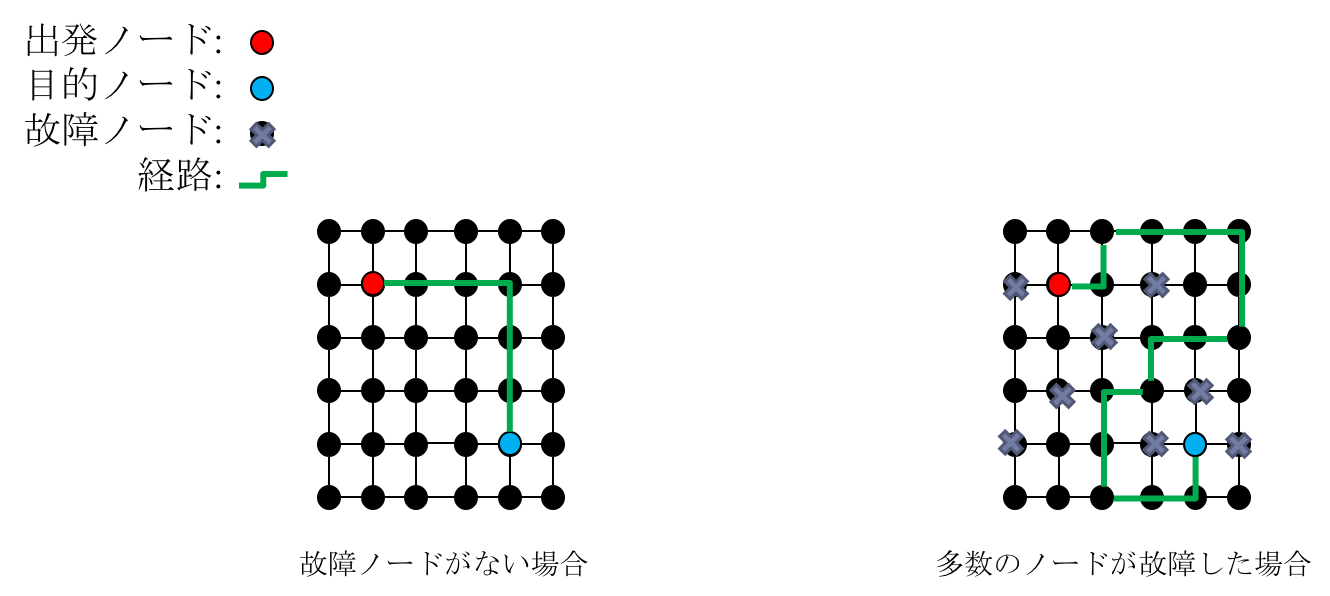
\includegraphics[width=12cm]{faulttolerant}
\caption{耐故障経路選択}
\label{fig:faulttolerant}
\end{figure}

また, ノード間通信を行う際にはなるべく短時間で通信を行うことが望ましいのは自明である. 
しかし, 単一通信経路の速度向上は物理的な限界があるため可能な限り並列な複数経路を確保することで
通信速度向上を達成することができる. 図\ref{fig:parallelpaths}にノード間で並列通信経路が確保された様子を示す.

\begin{figure}[htb]
\centering
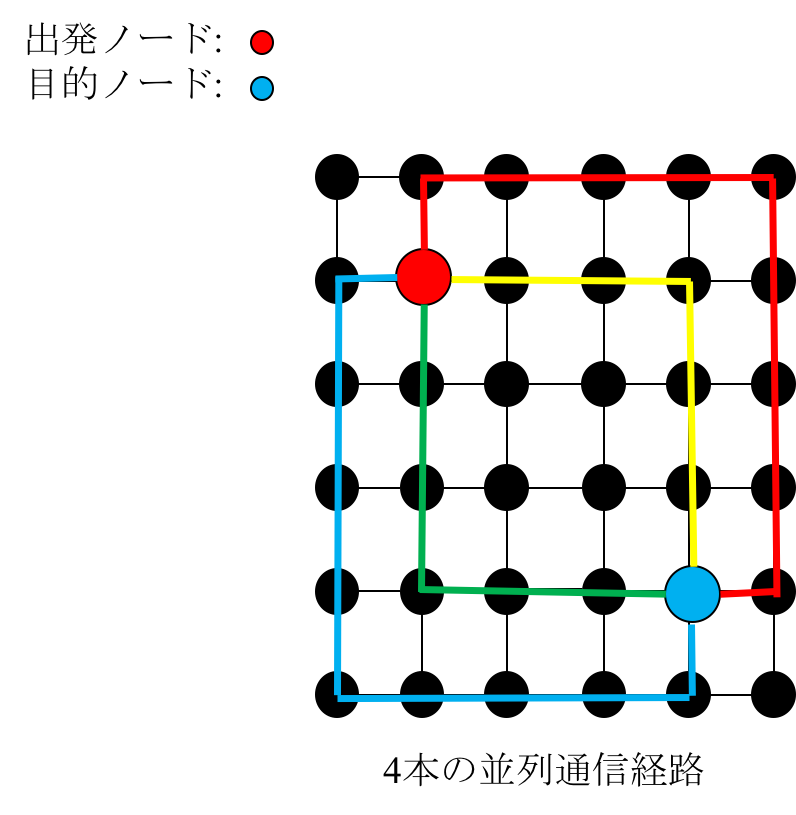
\includegraphics[width=8cm]{parallelpaths}
\caption{並列通信経路確保}
\label{fig:parallelpaths}
\end{figure}

上記図で示したとおり, 各ノードを頂点にノード間のリンクを辺で表現することでグラフ理論として問題を扱うことができる.
そして, 上記二つの問題は素な経路選択問題を解くことで解決することが可能になる. 素な経路選択問題は下記のような分類をすることができる.
\begin{itemize}
\item 頂点間素な経路選択
\item 頂点と頂点集合間素な経路選択
\item 頂点集合間素な経路選択
\item 頂点ペア間素な経路選択
\end{itemize}
まず, 素な経路とは複数の経路が同じ頂点を共有しないことである. 
そして頂点間素な経路選択は任意の2頂点間で複数の経路が経路の両端点を除き互いに素である場合, 
頂点と頂点集合間素な経路選択は任意の出発頂点と目的頂点集合間の複数の経路が出発頂点を除き互いに素である場合,
頂点集合間素な経路選択は任意の出発頂点集合と目的頂点の集合間の複数の経路が互いに素である場合である.
最後に頂点ペア間素な経路選択とは出発頂点と目的頂点のペア複数与えられた場合それらペア間の経路が互いに素である場合である.
図\ref{fig:disjointpaths}にこれらの例を示す.

\begin{figure}[htb]
\centering
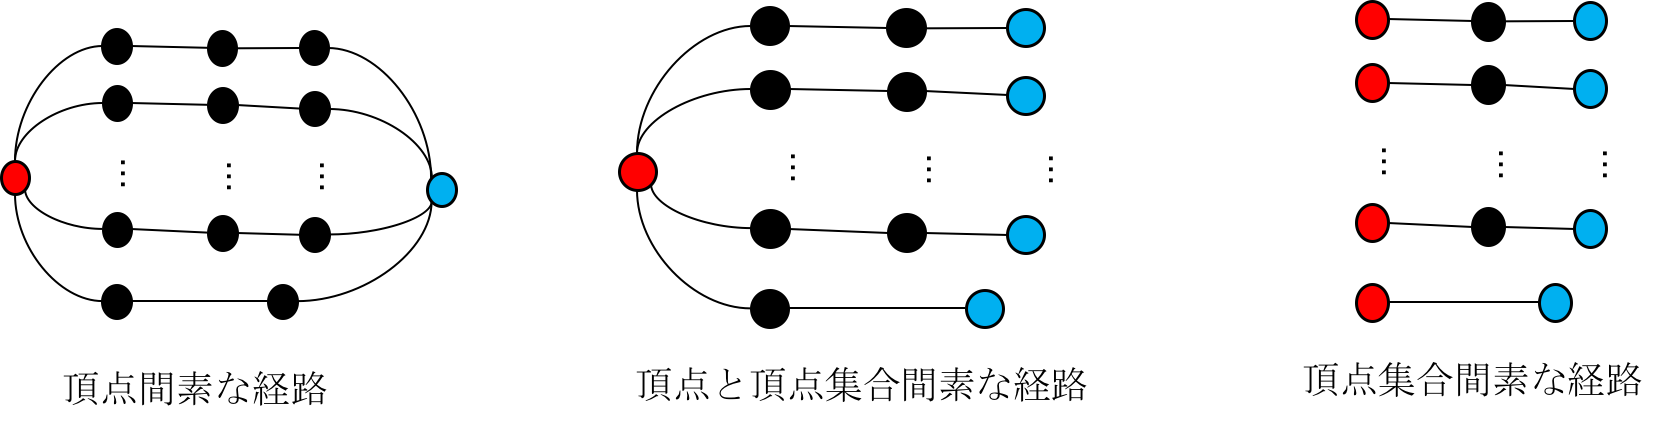
\includegraphics[width=14cm]{disjointpaths}
\caption{素な経路の種類}
\label{fig:disjointpaths}
\end{figure}



\end{document}